\documentclass{../source/Experiment}

\major{信息工程}
\name{姚桂涛}
\title{Cache Controller的设计}
\stuid{3190105597}
\college{信息与电子工程学院}
\date{\today}
\lab{}
\course{计算机组成与设计}
\instructor{沈继忠、赵武锋}
\grades{}
\expname{Cache Controller的设计}
\exptype{设计仿真}
\partner{}
\begin{document}
    \makecover
    \makeheader
    \section{实验任务}
    使用Verilog HDL设计一个一级数据缓存控制器(first-level  data  cache  controller)。
    \section{设计思路}
        \subsection{状态编码}
            参考教材5.9节,可以设计四个状态,分别为:
            \begin{figure}[H]
                \centering
                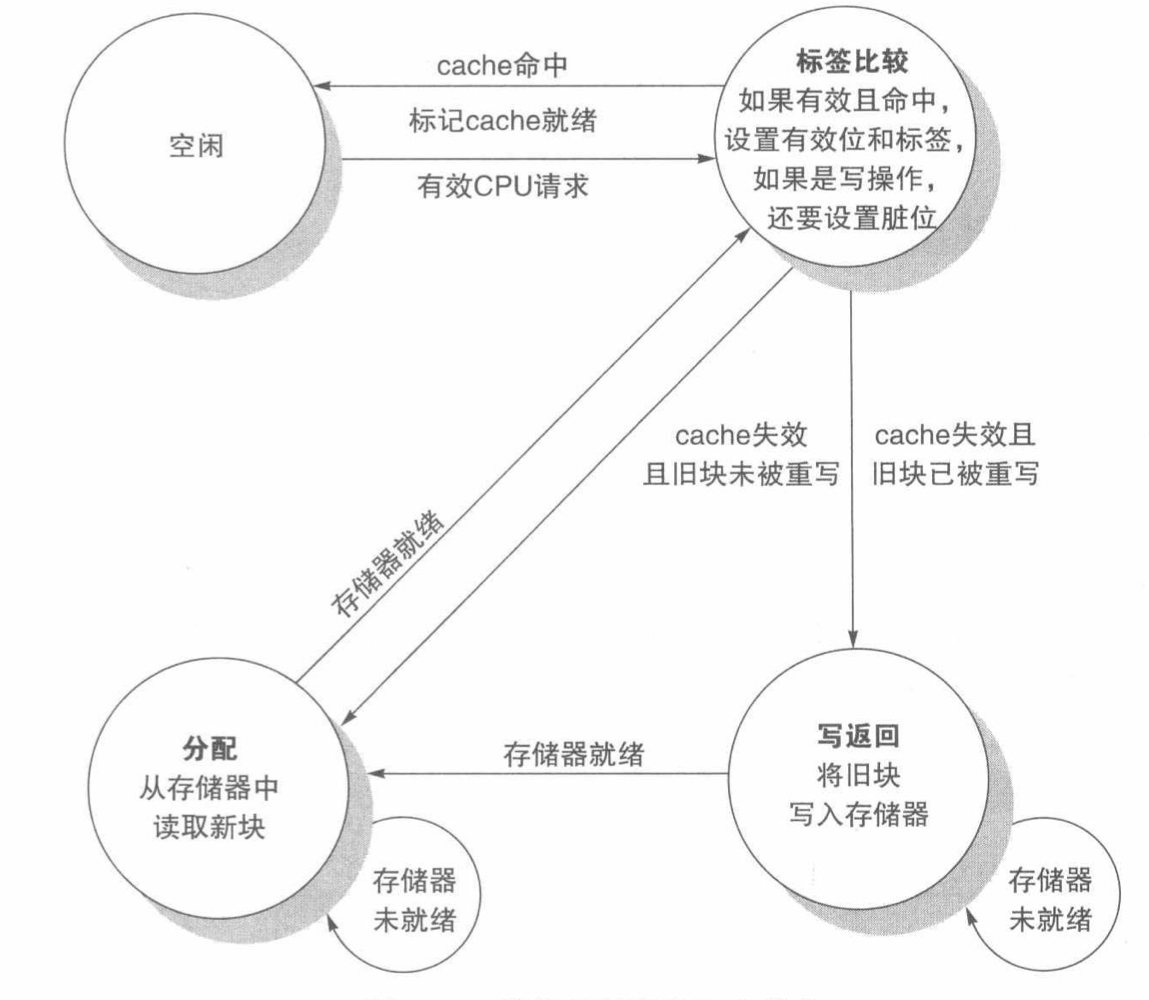
\includegraphics[width = 0.6\textwidth]{参考}
                \caption{控制器的四个状态}
            \end{figure}

            Idle:该状态等待处理器发出的有效读或写信号,之后有限状态自动机跳转到标签比较状态。

            CompareTag:正如名称所示,该状态检测读或写请求是命中还是失效。地址的索引部分选择用于比较的标签。如果地址中的索引部分引用的 cache 块中的数据是有效的,并且地址中的标签部分与标签相匹配,则命中。如果是加载指令就从选择的字中读取数据,如果是存储指令就将数据写人选择的宇中。之后设置 cache 就绪信号。如果这是个写操作,脏位还要设置为 1。需要注意的是,写命中也需要设置有效位和标签字段,即使这看上去并不需要。这是因为标签使用单独的存储器,因此在改变脏位时也需要同时改变有效位和标签字段。如果发生命中并且当前块是有效的,有限状态自动机会返回空闲状态。失效时先更新 cache 标签,之后如果当前块的脏位为 1,则跳转到写回状态,如果该位为 0,则跳转到分配状态。

            WriteBack:该状态使用由标签和 cache 索引组成的地址将 128 位的块写回存储器。之后继续停留在该状态等待存储器发出就绪信号。等待存储器写操作完成后,有限状态自动机跳转到分配状态。

            Allocate:从存储器中取出一个新块。之后继续停留在该状态等待存储器发出就绪信号。等待存储器读操作完成后,有限状态自动机跳转到标签比较状态。尽管我们可以不重新使用标签比较状态而跳转到一个新的状态完成操作,但是分配状态之后的操作与标签比较状态的操作有大量的重香,包括当访问为写操作时更新块中相应的宇。

            并对四个状态状态编码为Idle = 0 , CompareTag = 1 , WriteBack = 2 , Allocate = 3。
            
        \subsection{状态转换表}
            写出状态转移表如下表,“-”表示在当前状态转移情况下不关心该信号。
            \begin{table}[H]
                \begin{tabular}{|c|c|c|c|c|c|c|c|c|}
                \hline
                state                       & ld & st & addr{[}31:11{]} == tag & valid & dirty & l2\_ack & write\_done & nextstate                   \\ \hline
                \multirow{4}{*}{Idle}       & 0  & 0  & -                      & -     & -     & -       & -           & Idle                        \\ \cline{2-9} 
                                            & 0  & 1  & -                      & -     &       & -       & -           & \multirow{3}{*}{CompareTag} \\ \cline{2-8}
                                            & 1  & 0  & -                      & -     &       & -       & -           &                             \\ \cline{2-8}
                                            & 1  & 1  & -                      & -     &       & -       & -           &                             \\ \hline
                \multirow{3}{*}{CompareTag} & -  & -  & -                      & 0     & 0     & -       & -           & Allocate                    \\ \cline{2-9} 
                                            & -  & -  & -                      & 0     & 1     & -       & -           & WriteBack                   \\ \cline{2-9} 
                                            & -  & -  & -                      & 1     &       & -       & -           & Idle                        \\ \hline
                \multirow{2}{*}{WriteBack}  & -  & -  & -                      & -     & -     & -       & 0           & WriteBack                   \\ \cline{2-9} 
                                            & -  & -  & -                      & -     & -     & -       & 1           & Allocate                    \\ \hline
                \multirow{2}{*}{Allocate}   & -  & -  & -                      & -     & -     & 0       & -           & Allocate                    \\ \cline{2-9} 
                                            & -  & -  & -                      & -     & -     & 1       & -           & CompareTag                  \\ \hline
                \end{tabular}
            \end{table}
        \subsection{FSM流程图}
            利用drawio绘制出FSM流程图如图所示。
            \begin{figure}[H]
                \centering
                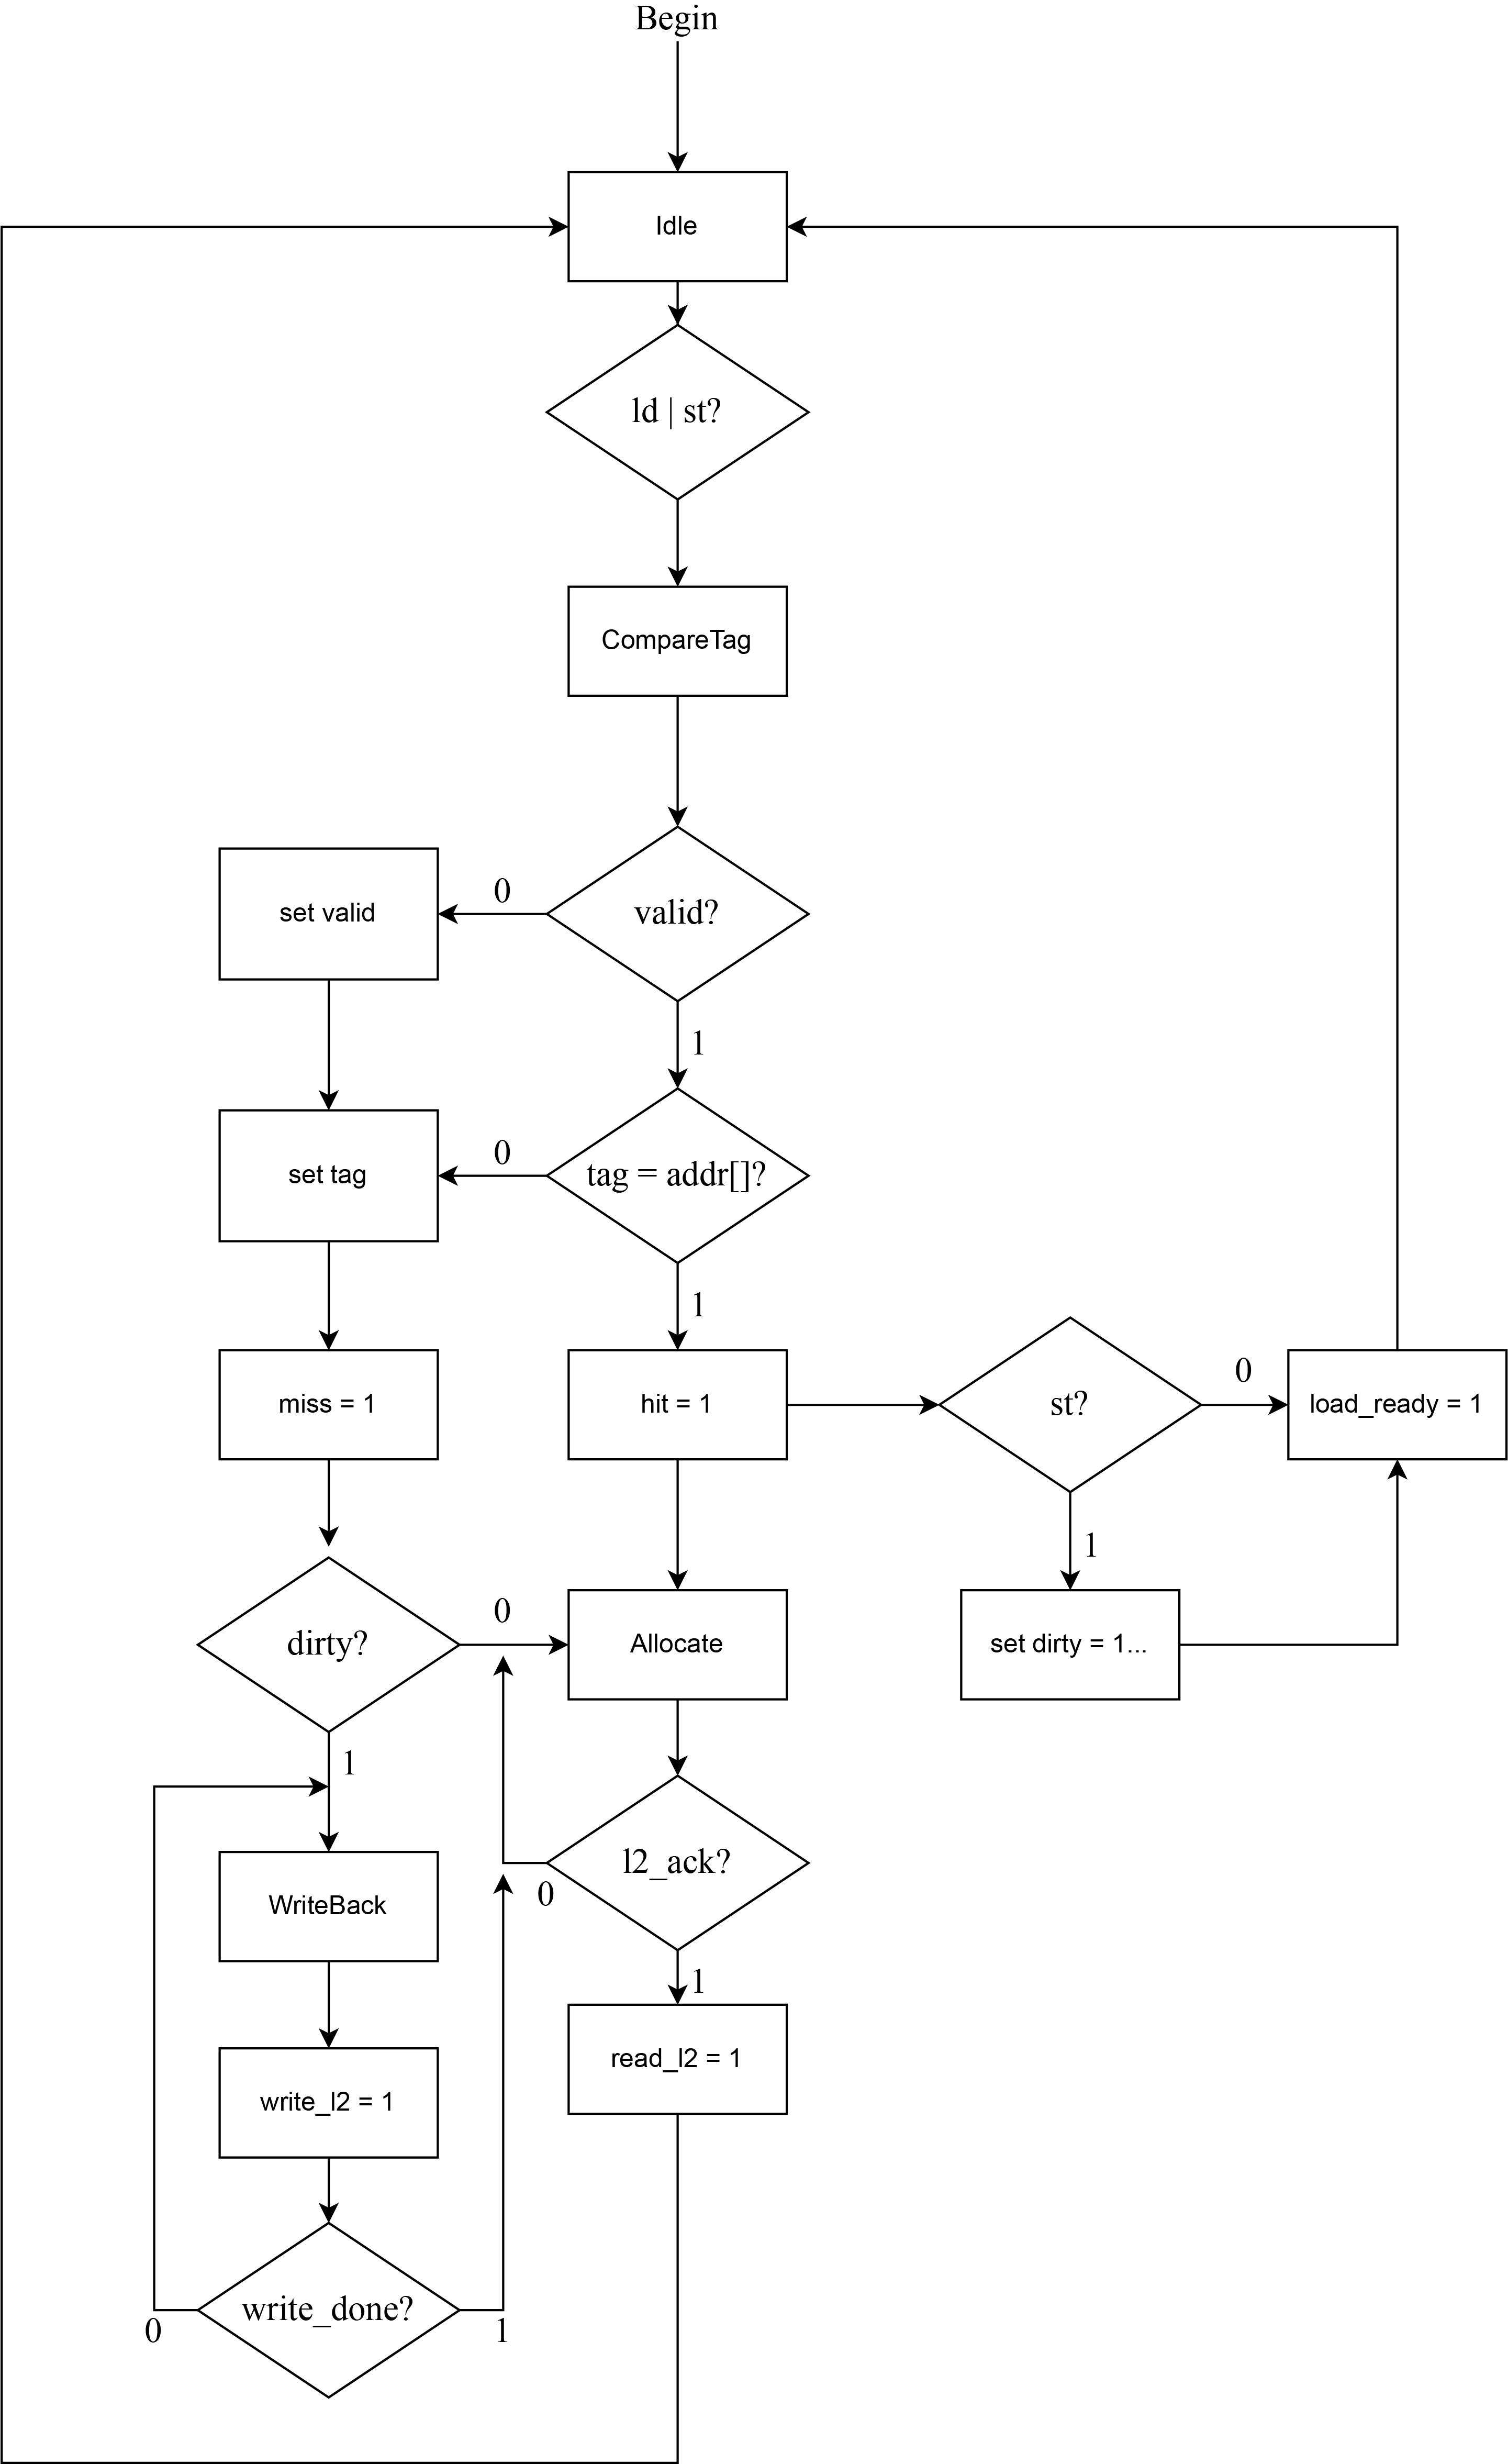
\includegraphics[width = 0.6\textwidth]{FSM}
                \caption{FSM流程图}
            \end{figure}
    \section{电路设计}
        通过vivado软件进行电路设计,如下图
        \begin{figure}[H]
            \centering
            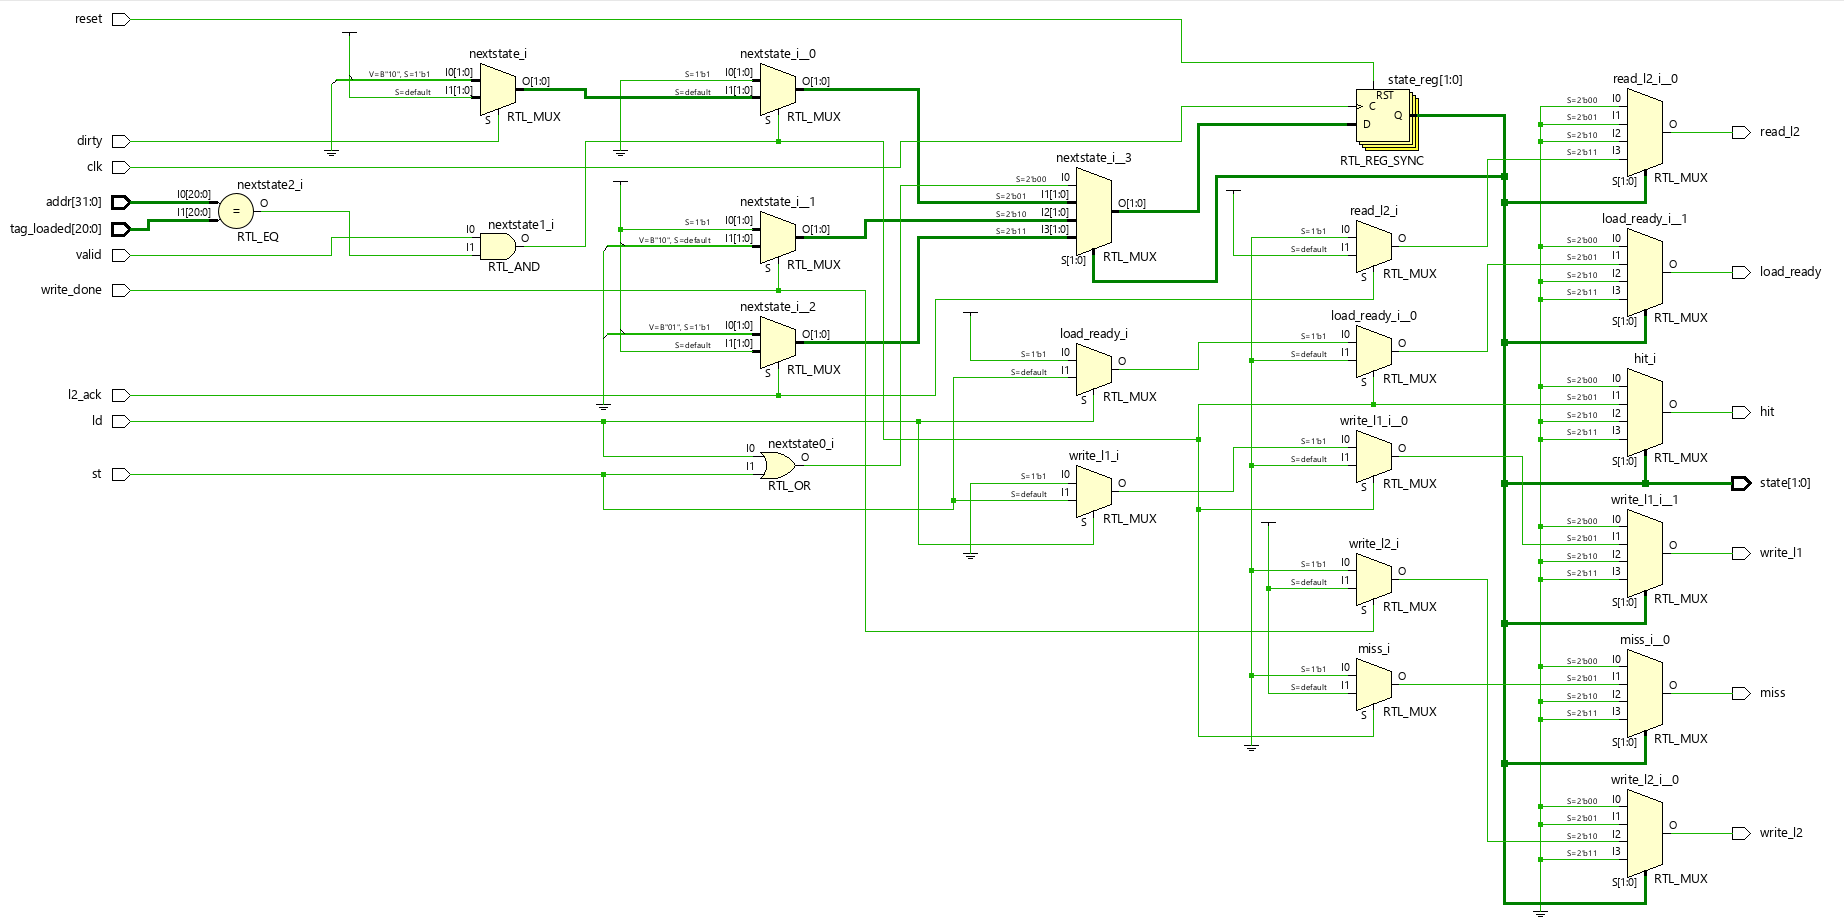
\includegraphics[width = 1\textwidth]{RTL}
            \caption{电路图}
        \end{figure}
    \section{主要仪器设备}
        装有vivado的计算机,
    \section{Verilog设计与仿真}
        \subsection{代码实现}
            \subsubsection{cache控制器代码}
            \lstinputlisting[
                language  =   Verilog,
            ]{proj2/oddyti/CacheController.v}

            \subsubsection{仿真测试代码}
            `timescale 1ns / 1ps
            \lstinputlisting[
                language  =   Verilog,
            ]{proj2/oddyti/CacheController_tb.v}

        \subsection{测试结果}
            \begin{figure}[H]
                \centering
                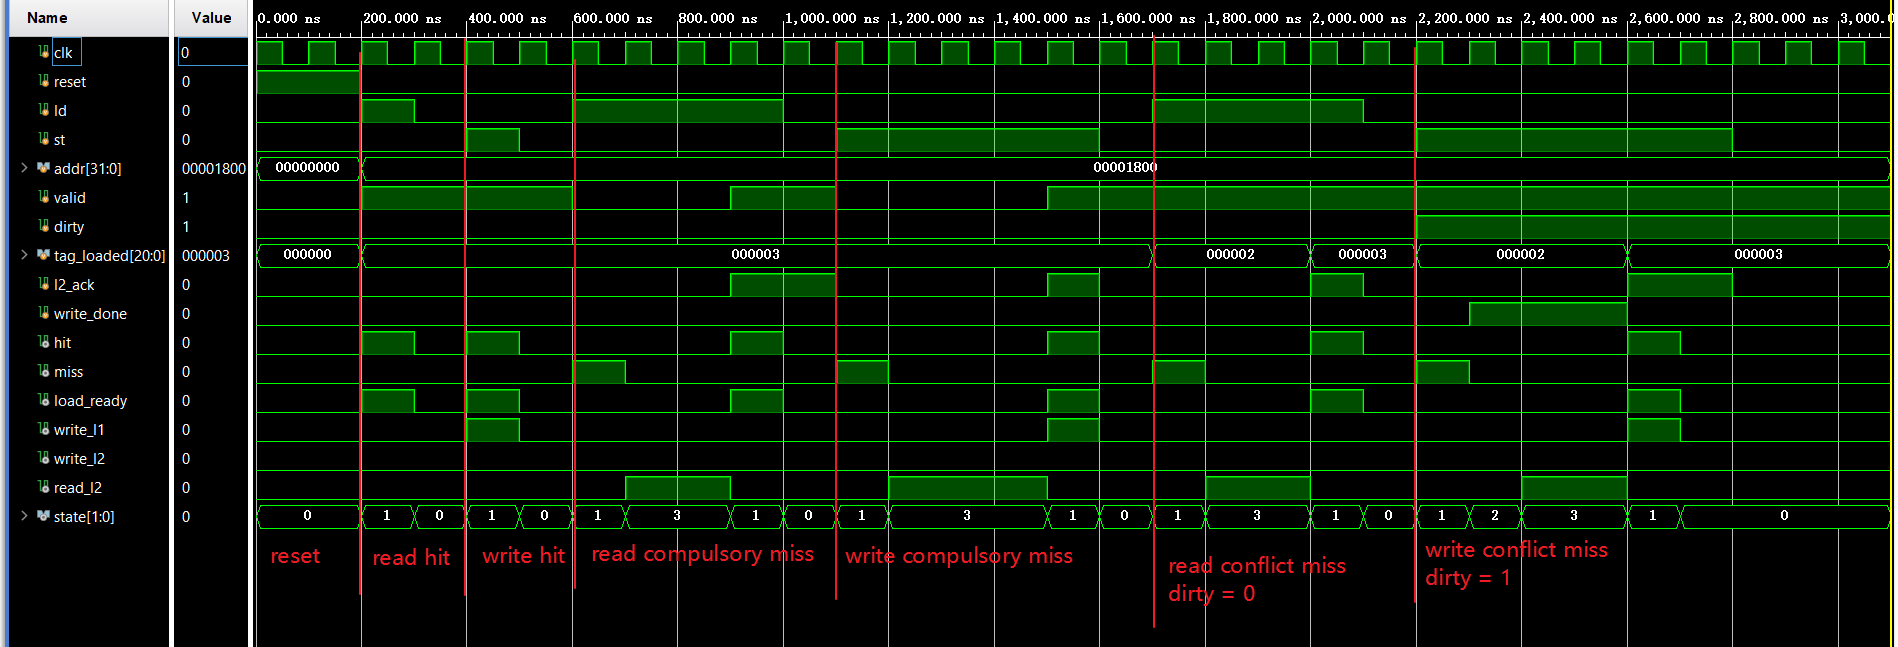
\includegraphics[width = 1\textwidth]{结果}
                \caption{测试结果}
            \end{figure}
        观察测试结果仿真图,可以看出控制信号正确。

    \section{心得体会}
        通过本次实验,我对cache有了更加深入的理解。同时本次实验的测试文件是自己编写的,是自己第一次编写,也学会了许多。

\end{document}